\chapter{Betrieb}

\section{Wichtige Daten}

\subsection{Unternehmensstruktur}

\begin{figure}[H]
    \centering
    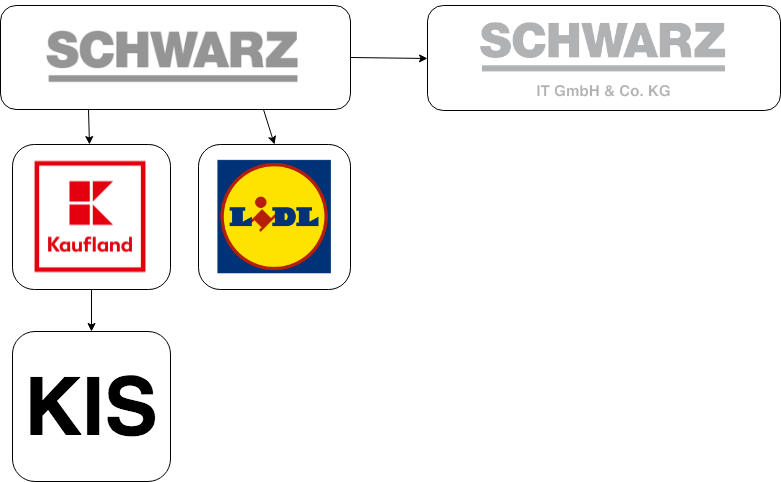
\includegraphics[width=\textwidth]{include/images/Unternehmensstruktur.png}
    \caption{Unternehmensstruktur Schwarzgruppe}
    \small Kaufland Informationssysteme ist Teil von Kaufland und Kaufland ist teil der Schwarzgruppe
    \label{fig-Schwarzgruppe}
\end{figure}


Es ist das Ziel möglichst viele Bereiche von Kaufland und KIS in der Schwarzgruppe allgemein und bei KIS in der SIT zu zentralisieren, um durch Zusammenarbeit von Kaufland und Lidl einen effizienteren Arbeitsprozess zu ermöglichen. 

\subsection{Unternehmensgeschichte}

-> siehe Kaufland Chronik 

\subsection{Nett to know}

Kaufland ist mit über 1200 Filialen und über 150.000 Mitarbeitern in 6 Ländern vertreten und strebt die Expansion nach Moldawien (2018) und Australien (2020) an. Kaufland unterhält 17 Logistikzentren und 4 Fleischwerke. Darüber hinaus betreibt Kaufland die            K-Classic, Exquisit und Purland Eigenmarken und bietet im Rahmen von Kaufland Reisen Reisen an. Dadurch, dass Kaufland sich auf ein Breites Sortiment ausgerichtet hat, gibt es in einem Markt bis zu 60.000 Artikel. 

\subsection{Mein Praktikumsstandort}

Ich habe mein Praktikum bei der Kaufland Informationssysteme GmbH \& Co. KG (KIS) in der Hallerstraße 59 in Weinsberg absolviert. Dort war ich im Bereich der Anwendungsentwicklung und in der Abteilung Java-Developement eingesetzt. Einige Termine fanden auch im benachbarten Gebäude der Schwarz IT GmbH \& Co. KG (SIT) statt, da beide Firmen zur Schwarzgruppe gehören und diverse Abteilungen schon in die SIT überführt wurden und da der Westflügel des KIS-Gebäudes renoviert wird, werden die Räumlichkeiten der SIT mitbenutzt. 

\section{KIS}

Die zwei wichtigsten Bereiche der KIS sind das Business Consulting (BC) und die Anwendungsentwicklung (AE). Die Business Consultants vermitteln zwischen Fachbereichen (FB) und Anwendungsentwicklung. Die Fachbereiche geben an die BCs weiter, welche Fehler es gibt oder was optimiert werden kann, der BC überlegt sich dann wie das Problem gelöst werden kann und wendet sich an einen Anwendungsentwickler, der dann eine Lösung ausarbeitet. Je nachdem um welchen Fachbereich es sich handelt und welches Problem gelöst werden muss sind verschiedene AEs zuständig. Natürlich gibt es über diese zwei hinaus noch weitere Bereiche, die ich aber jetzt vernachlässige, da sie bei der zentralen Dienstleistung, der IT-Lösung, nicht direkt in Verbindung stehen. Allerdings sind diese Bereiche trotzdem wichtig um sich z. B. um das Personal zu kümmern.